\begin{frame}{Ярусно-параллельная форма графа (ЯПФ)}

ЯПФ — это представление графа алгоритма, в котором:

% \begin{itemize}
%     \item ЯПФ — это представление графа алгоритма, в котором:
    
    \begin{itemize}
        \item все вершины разбиты на перенумерованные подмножества ярусов; 
        \item начальная вершина каждой дуги расположена на ярусе с номером меньшим, чем номер яруса конечной вершины;
        \item между вершинами, расположенными на одном ярусе, не может быть дуг.
    \end{itemize}

%     \item Высота ЯПФ — это число ярусов. Минимальной высотой всех возможных ЯПФ графа является его критический путь.
    
%     % \item Канонической ярусно-параллельной формой называется ЯПФ, высота которой на единицу больше длины критического пути, а все входные вершины расположены на первом ярусе. Для заданного графа его каноническая ЯПФ единственна. Высота канонической ЯПФ соответствует параллельной сложности алгоритма.

% \end{itemize}

% Высота ЯПФ — это число ярусов. Минимальной высотой всех возможных ЯПФ графа является его критический путь.
\end{frame}

% длинное тире: —


\begin{frame}{Пример выделения ЯПФ на двумерном графе}
\vspace{4mm}
\begin{columns}

% \begin{column}{0.25\textwidth}

% 123

% \end{column}

\begin{column}{0.25\textwidth}
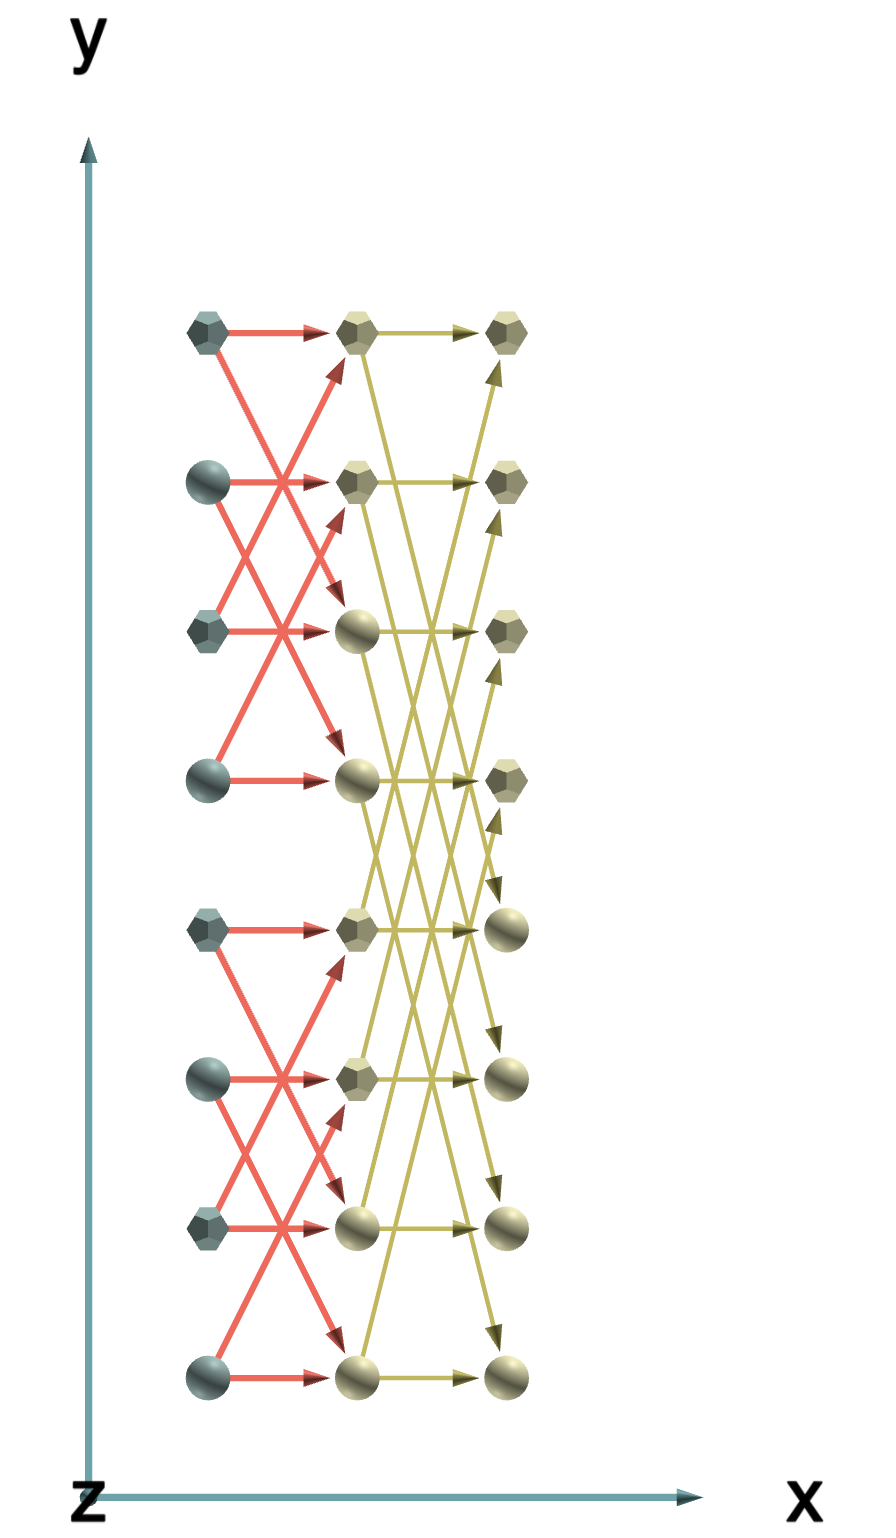
\includegraphics
[width=\textwidth]{animated/foo-1}\\
% Подсветка 1 яруса
% Highlighting 1st level
Level 1 marking
\end{column}

\begin{column}{0.25\textwidth}
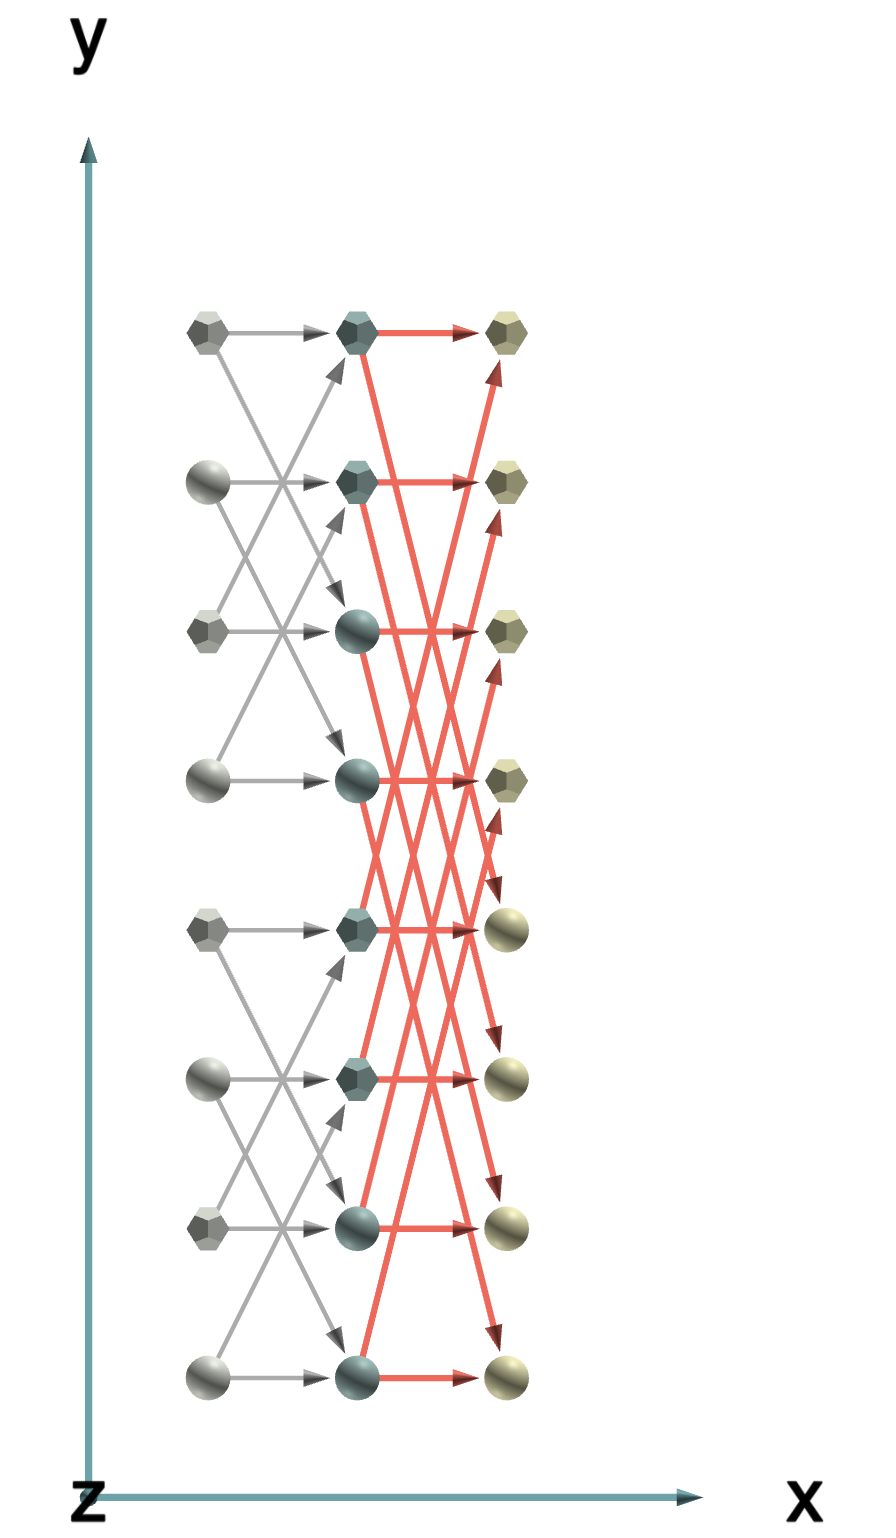
\includegraphics
[width=\textwidth]{animated/foo-2}\\
% Подсветка 2 яруса
Level 2 marking
\end{column}

\begin{column}{0.25\textwidth}
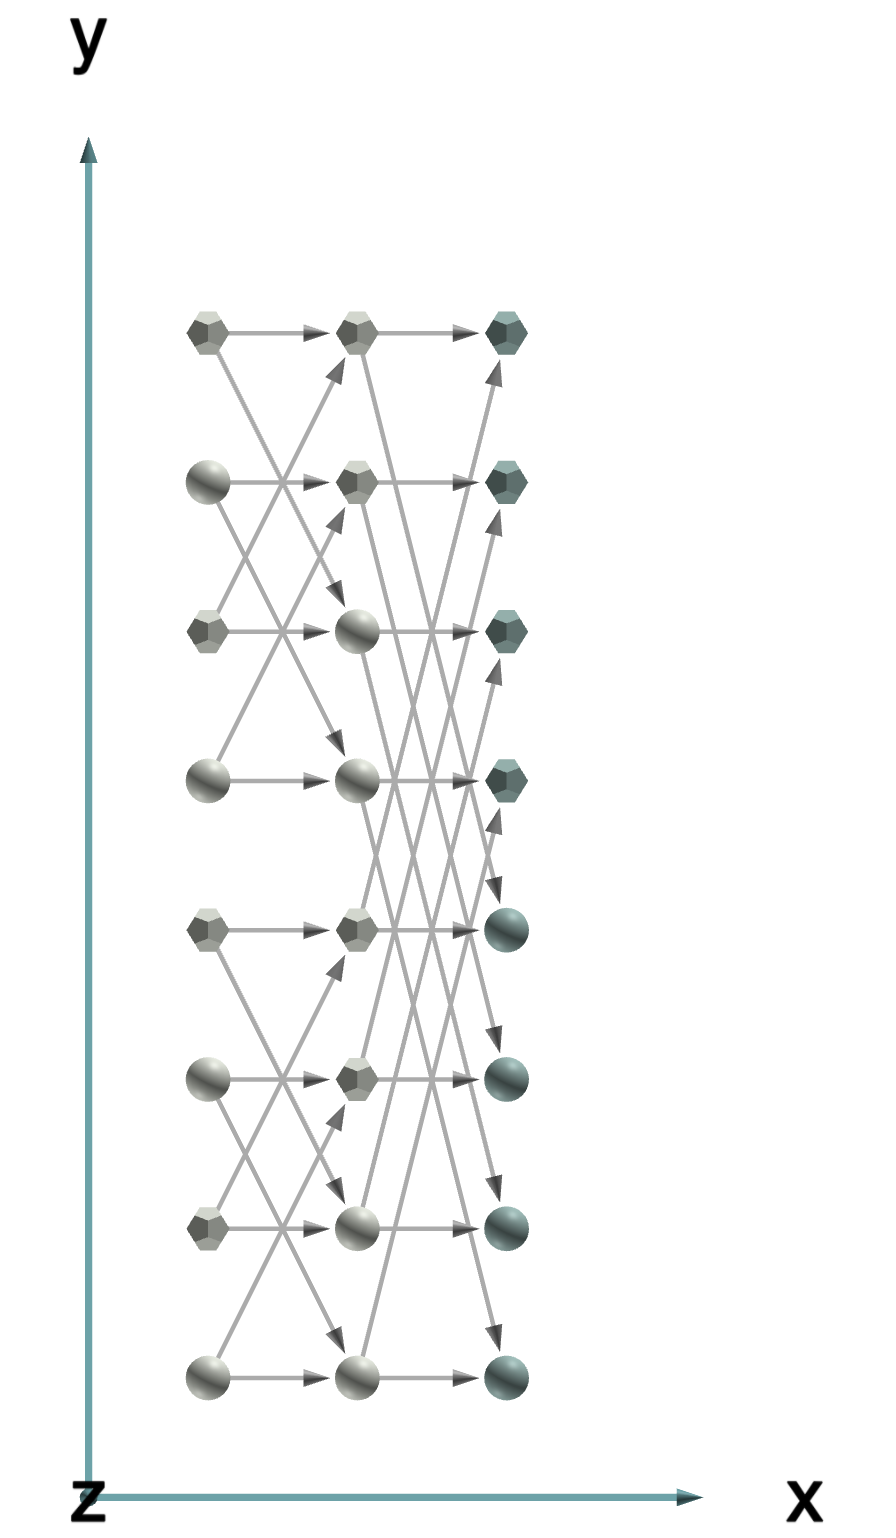
\includegraphics
[width=\textwidth]{animated/foo-3}\\
% Подсветка 3 яруса
Level 3 marking
\end{column}

\end{columns}
\end{frame}
